\definecolor{git}{RGB}{172, 49, 49}
\def\git#1{{\small\color{git}\$ git #1}\\}

\begin{frame}[fragile]{Why not just local git?}
  \begin{itemize}
  \item<1-> Local git alone via command line: Ok
  \item<2-> But lack of functionalities:
    \begin{itemize}
    \item User/permission management
    \item Bug tracking
    \item Duscussing implementations
    \item Forking other projects
    \item Easy collaborative development 
    \end{itemize}
  \item<3-> Several services were developed around git
    \begin{itemize}
    \item 
\includegraphics[width=15px]{images/GitHub-Mark.png} GitHub \url{https://github.com/}
    \item 
\includegraphics[width=15px]{images/bitbucket.png} bitbucket \url{https://bitbucket.org/}
    \item 
\includegraphics[width=15px]{images/GitLab_Logo.png} GitLab \url{https://git.framasoft.org/}
    \item ...
    \end{itemize}
  \end{itemize}
\end{frame}

\begin{frame}{GitHub}
  \begin{itemize}
  \item url : https://GitHub.com/ 
  \item 
\includegraphics[width=15px]{images/Wikipedia_logo.png} Wikipedia: GitHub is a web-based Git repository hosting service. It offers all of the distributed revision control and source code management (SCM) functionality of Git as well as adding its own features. Unlike Git, which is strictly a command-line tool, GitHub provides a Web-based graphical interface and desktop as well as mobile integration. It also provides access control and several collaboration features such as bug tracking, feature requests, task management, and wikis for every project.
  \end{itemize}
\end{frame}

\begin{frame}{GitHub: Use Case}
  \begin{itemize}
  \item Development of a piece of code with a collaborator
  \item Creating the project
  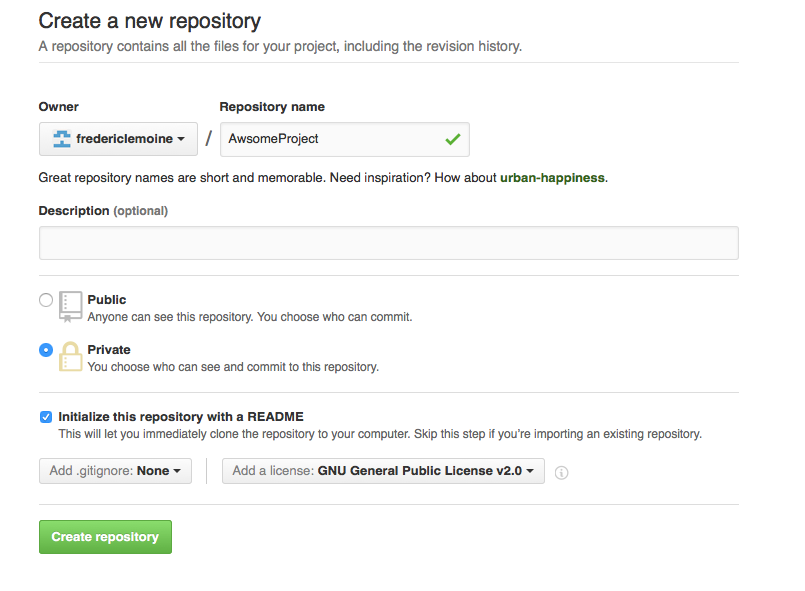
\includegraphics[width=0.8\textwidth]{images/hosting_services_use_case_1.png}
  \end{itemize}
\end{frame}

\begin{frame}{GitHub: Use Case - Project creation}
  \begin{itemize}
  \item Project created
    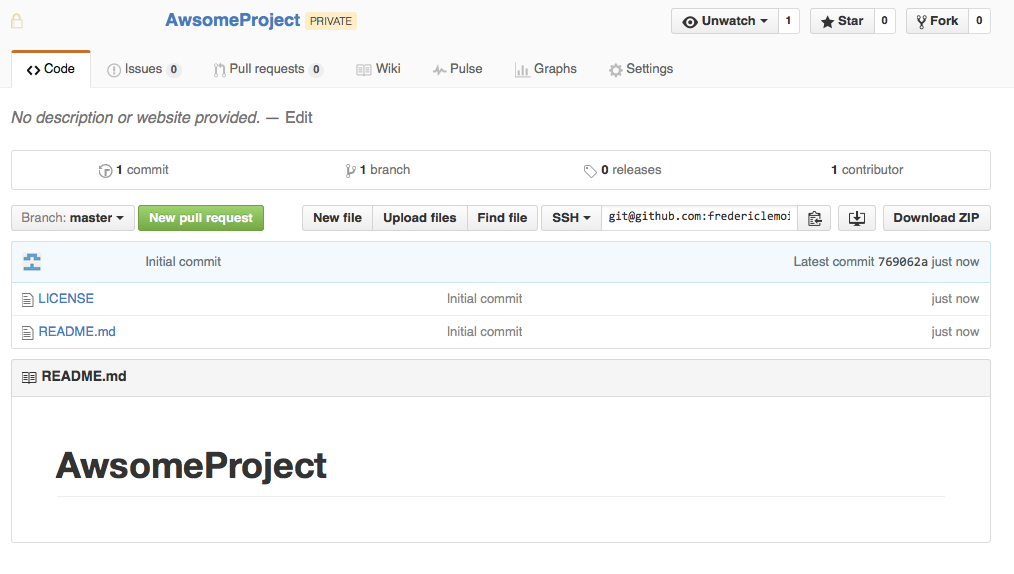
\includegraphics[width=\textwidth]{images/hosting_services_use_case_2.png}
  \end{itemize}
\end{frame}

\begin{frame}[fragile]{GitHub: Use Case - Adding code}
  \begin{itemize}
  \item cloning the project
  \end{itemize}
  \begin{lstlisting}
    $ git clone git@github.com:fredericlemoine/AwsomeProject.git
    $ cd AwsomeProject
    $ ls
    -rw-r--r-- 1 flemoine staff 18K 10 avr 16:48 LICENSE
    -rw-r--r-- 1 flemoine staff  15 10 avr 16:48 README.md
  \end{lstlisting}
\end{frame}

\begin{frame}[fragile]{GitHub: Use Case - Adding code}
  \begin{itemize}
  \item Adding code
  \end{itemize}
  \begin{lstlisting}
    $ cat > myfristfile.pl
    while(<>){
      chomp;
      my @tab = split(/\t/);
      $tab[1]=~tr/acgt/ACGT/;
      print ">".$tab[0]."\n";
      print $tab[1]."\n";
    }
    $ git add myfristfile.pl
    $ git commit -m "My Frist perl unintelligible code"
    $ git push -u origin master
    \end{lstlisting}
\end{frame}

\begin{frame}{GitHub: Use Case - Code added}
  \begin{itemize}
  \item Code added
    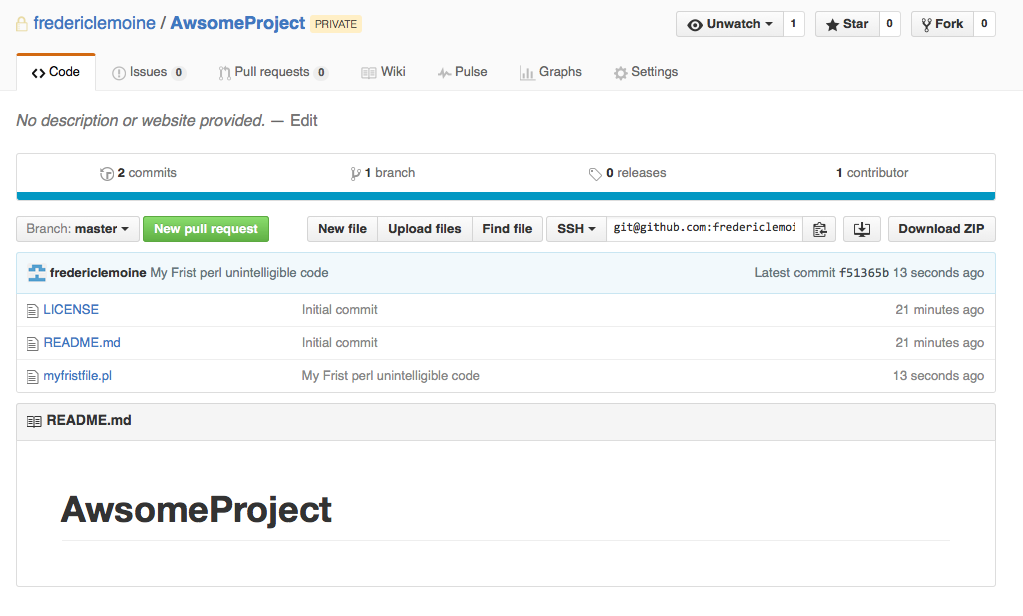
\includegraphics[width=\textwidth]{images/hosting_services_use_case_3.png}
  \end{itemize}
\end{frame}

\begin{frame}{GitHub: Use Case - Someone proposes a modification}
  \begin{itemize}
  \item New branch on GitHub
    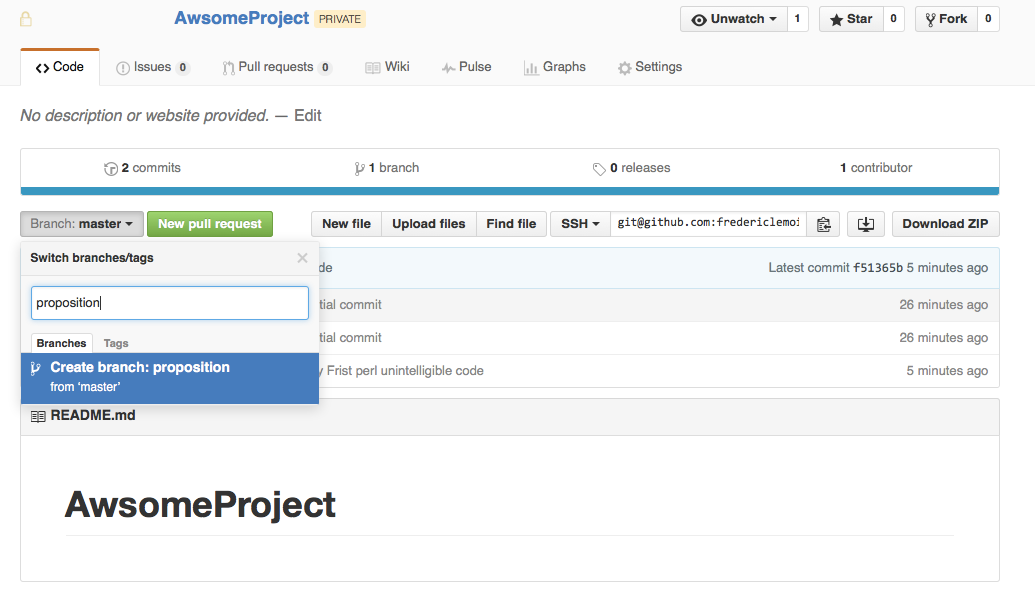
\includegraphics[width=\textwidth]{images/hosting_services_use_case_4.png}
  \end{itemize}
\end{frame}

\begin{frame}[fragile]{GitHub: Use Case - Someone proposes a modification}
  \begin{itemize}
  \item Modification
    \begin{lstlisting}
      $ git fetch
      $ git checkout proposition
      $ emacs myfristfile.pl
      $ git diff myfristfile.pl
      diff --git a/myfristfile.pl b/myfristfile.pl
      index 9b49709..575c418 100644
      --- a/myfristfile.pl
      +++ b/myfristfile.pl
      @@ -1,6 +1,6 @@
      while(<>){
        my @tab = split(/\t/);
        -  $tab[1]=s/[acgt]/ACGT/g;
        -  $tab[1]=~tr/acgt/ACGT/;
        +  $tab[1]=~tr/acgtu/ACGTU/;
        print ">".$tab[0]."\n";
        print $tab[1]."\n";
      }
      $ git add myfristfile.pl
      $ git commit -m "Modification of nucleotides"
      $ git push -u origin proposition
    \end{lstlisting}
  \end{itemize}
\end{frame}

\begin{frame}[fragile]{GitHub: Use Case - Someone proposes a modification}
  \begin{itemize}
  \item Pull request
    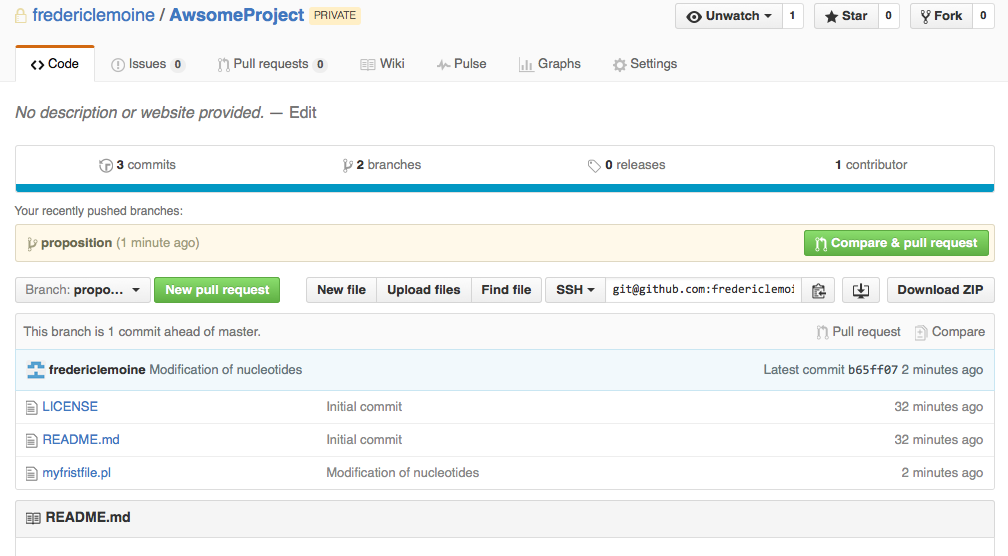
\includegraphics[width=\textwidth]{images/hosting_services_use_case_5.png}
  \end{itemize}
\end{frame}

\begin{frame}[fragile]{GitHub: Use Case - Someone proposes a modification}
  \begin{itemize}
  \item Pull request
    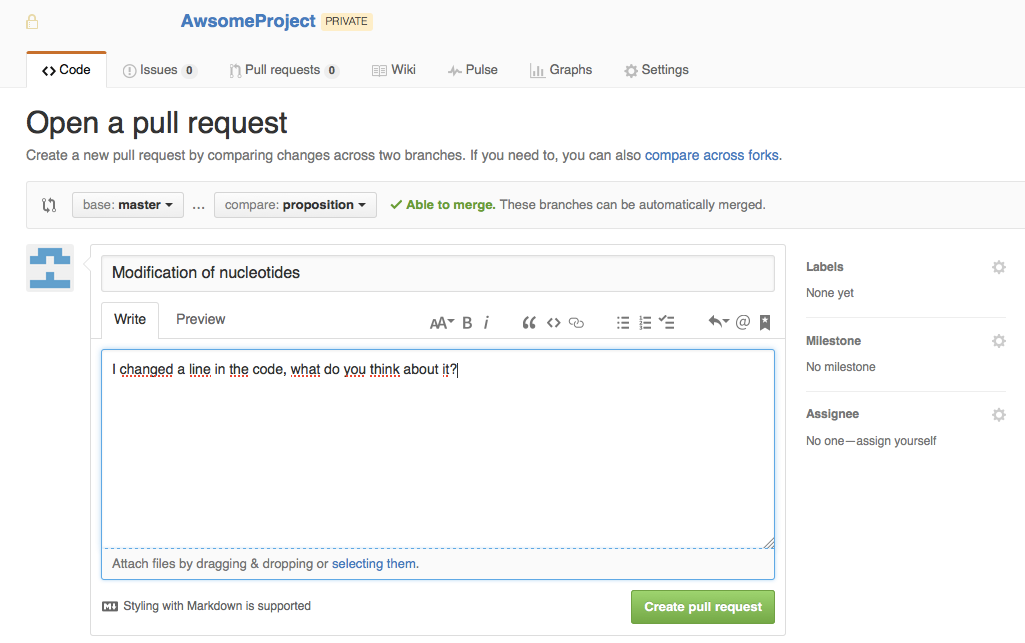
\includegraphics[width=\textwidth]{images/hosting_services_use_case_6.png}
  \end{itemize}
\end{frame}

\begin{frame}[fragile]{GitHub: Use Case - Someone proposes a modification}
  \begin{itemize}
  \item Pull request
    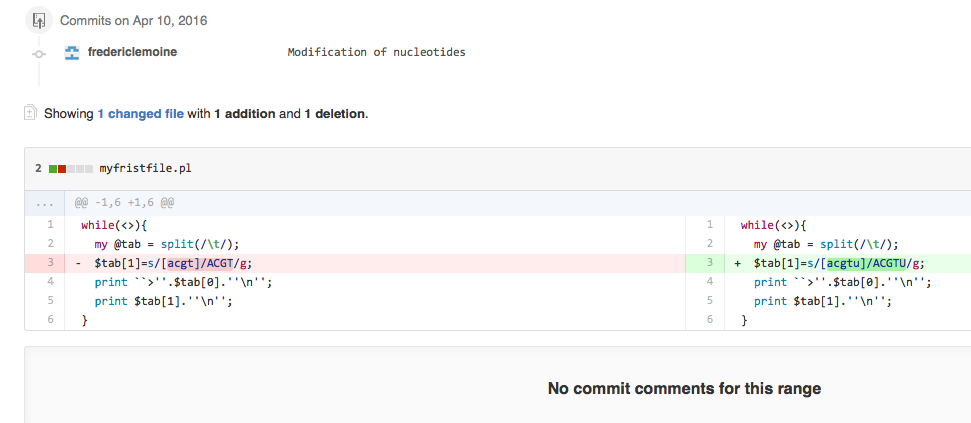
\includegraphics[width=\textwidth]{images/hosting_services_use_case_7.png}
  \end{itemize}
\end{frame}

\begin{frame}[fragile]{GitHub: Use Case - Someone proposes a modification}
  \begin{itemize}
  \item Pull request
    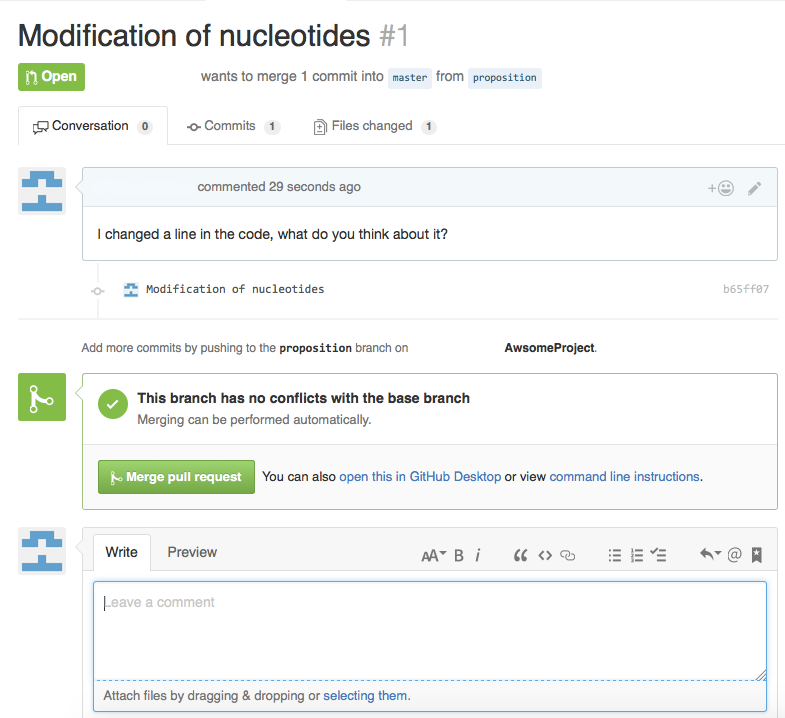
\includegraphics[width=\textwidth]{images/hosting_services_use_case_8.png}
  \end{itemize}
\end{frame}


\begin{frame}[fragile]{GitHub: Use Case - Before merging}
  \begin{itemize}
  \item Modification in master
    \begin{lstlisting}
      $ git checkout master
      $ emacs README.md
      $ git add README.Md
      $ git commit -m "Modification of README"
      $ git push -u origin master
    \end{lstlisting}
  \item THEN accept pull request and delete proposition branch
  \end{itemize}
\end{frame}

\begin{frame}[fragile]{GitHub: Use Case - After merging}
  \begin{itemize}
  \item Network of branches
    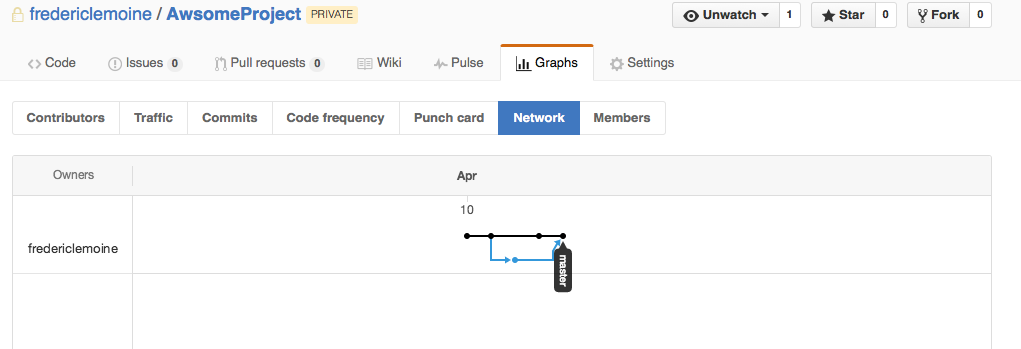
\includegraphics[width=\textwidth]{images/hosting_services_use_case_9.png}
  \end{itemize}
\end{frame}


\begin{frame}[fragile]{GitHub: Use Case - Tesing!}
  \begin{itemize}
  \item<1-> Is my code buggy?
  \item<2-> I want to test my code!
  \item<3-> 
\includegraphics[width=15px]{images/Travis_CI_Logo.png} Tavis CI
  \item<4-> Just write a YML file \verb+.tavis-ci.yml+
    \begin{lstlisting}
      language: perl
      perl:
      - "5.22"
      - "5.20"
      - "5.18"
      - "5.16"
      - "5.14"
      before_install: true
      install: true
      before_script: true
      script:
      - echo -e "SEQ1\tacgt\tcol2\tcol3" | perl myfristfile.pl
    \end{lstlisting}
  \item<5-> Then
    \begin{lstlisting}
      $ git add .travis-ci.yml
      $ git commit -m "Travis CI"
      $ git push
    \end{lstlisting}
  \end{itemize}
\end{frame}



\begin{frame}[fragile]{Travis CI}
  \begin{itemize}
  \item After each push on GitHub, a Travis CI build is triggered automatically
  \item After the build, the result is sent by e-mail
  \item Web interface
    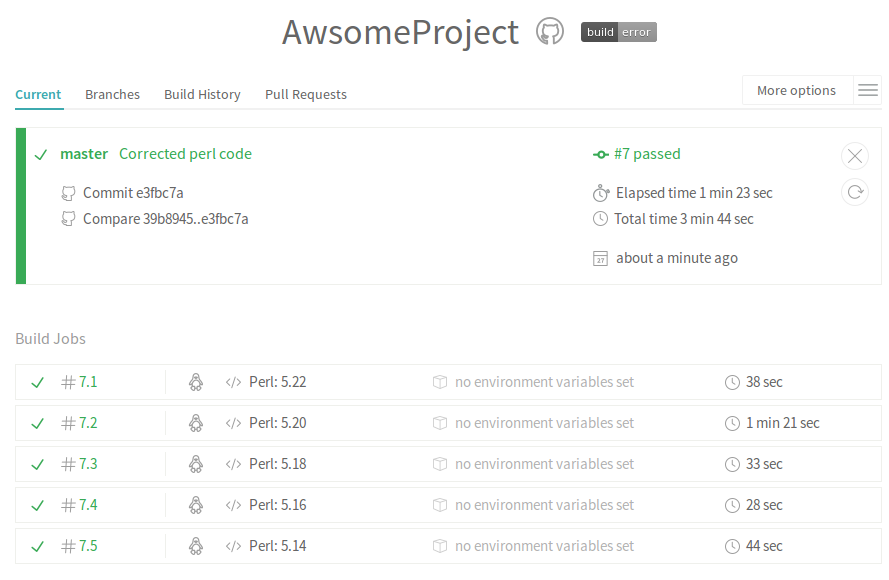
\includegraphics[width=0.8\textwidth]{images/hosting_services_use_case_10.png}
  \end{itemize}
\end{frame}

\begin{frame}[fragile]{Travis CI}
  \begin{itemize}
  \item Result logs
    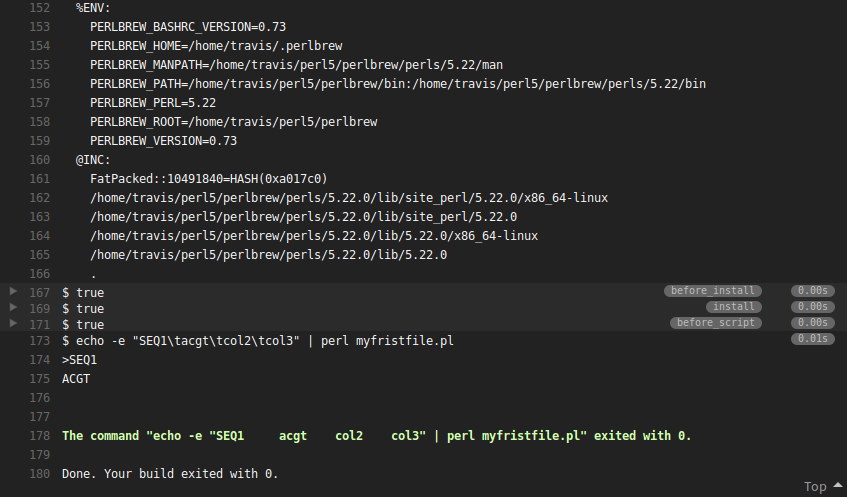
\includegraphics[width=0.8\textwidth]{images/hosting_services_use_case_11.png}
  \end{itemize}
\end{frame}


